\newpage


\section{Persistent storage}
\label{sec:persistentStorage}

% Problem statement
A fault-tolerant decentralised design can be beneficial with regards to data availability in a service where information needs to be stored. By introducing data maintenance mechanisms we can make information persist beyond an instance of a specific node. Trivially, if there is no possibility of node or link failure, a node can simply transfer the information it hosts to another node before gracefully exiting the network. However, if we introduce the possibility of failure, maintaining a high probability of data retention becomes significantly more challenging.\cite{shinebourne2022availability}

% Without data replication, information availability is dependent on the availability of any given node.
An obvious solution to making data persist despite failure is to introduce a certain level of information redundancy on the network. However, efficiently managing redundant copies of information is a non-trivial challenge. If the network has a high churn rate, i.e.\ a high turnover of nodes either gracefully or ungracefully (by failure) leaving the network, this problem becomes highly relevant\cite{duarte2014reliable, ranganathan2002replication}.

% Contribution
In this module of Butter, an overlay network was designed based on the premise of Peer Content Groups (PCGs)\cite{duarte2014reliable}. The original design was first modified to remove reliance on structured network elements\cite{shinebourne2022availability, duarte2014reliable}, and here we suggest further extensions to the protocols, improving the performance of the data retention mechanism while maintaining a decentralised design and usable levels of efficiency.

\subsection{Related work}

In this section we will explore some of the existing approaches and technologies that enable persistent storage of information on a peer-to-peer network.

\subsubsection{Peer Content Groups (PCGs)}
\label{sssec:pcgAvailability}

Peer Content Groups provide an intuitive framework for reasoning about persistent information on a network. Instead of thinking about data in terms of individual nodes, we think about data being hosted by logical entities known as PCGs. The original premise for PCGs was to allow for transparent interaction with the network. So, if a peer fulfilling a request fails, the request can still be handled by other members of its group. This puts the responsibility of the quality of service on the peer-to-peer network, rather than on the peer making the request\cite{shinebourne2022availability}.

The protocol is as follows: when information is added to the network, a group is created, hence, each group maintains one data block on the network, replicating it across its members\cite{shinebourne2022availability}. A node can be a member of as many groups as it has the memory capacity to store. The network of groups is `overlayed' on the network of Butter nodes. Members of the same group are not necessarily known hosts to each other, so, the PCG network may have different edges to the underlying known host network (see Figure~\ref{fig:overlayPCG}). Groups recruit new members through the use of advertisements, and a node may join a group by responding to an advertisement. Advertisements introduce the main limitation of the original PCG implementation\cite{duarte2014reliable}. In the original PCG protocol there is the notion of super-peers which work as rendezvous points where group advertisements are publicised. This enables efficient communication across the network. However, this reliance on super-peers, re-introduces elements of centralisation.

Groups know to advertise for new members based on their Group status. Each node maintains its own group status by the using heartbeat pings. The heartbeat pings are used as eventually perfect peer failure detectors, i.e.\ oracles that eventually output an accurate representation of what nodes have failed in the group. When a heartbeat message is received from a node, it updates its $localGroupView$, i.e.\ what each group member node believes to be the group’s state. If a node does not receive a heartbeat ping within a given timeout period, the peer is removed from the node’s view of the group members. This process allows the group status to tend towards consensus.\cite{shinebourne2022availability}

If the group is in an arbitrarily defined `unsafe' state, i.e.\ if the group is too low on members and hence the information it is responsible for is at relatively high risk of loss, a leader is elected to publish an advertisement at the rendezvous point. If available, a new node will join the group.

\subsubsection{The group membership problem}

As seen in Section~\ref{sssec:pcgAvailability}, it is required that PCGs maintain some consensus on the group status, i.e.\ what group members are still alive and hosting the group information. This allows the data to remain highly available despite node failure. The generalisation of this problem is introduced in Riccardi’s paper\cite{ricciardi1992gmp} as the Group Membership Problem (GMP). The GMP consists of two ideas: eventually perfect failure detection\cite{mostefaoui2003failure} and consensus\cite{barborak1993consensus} between non-faulty group members on current group member status\cite{bracha1985asynchronous}.

% Methods for achieving group membership
There are several methods that can be employed to achieve consensus between group members and hence have an accurate group status. Here we discuss two possible approaches: Heartbeat protocols and Randomised gossiping protocols.

\begin{itemize}
    \item \textbf{Heartbeat protocols}\\
    Heartbeat protocols are conceptually simple and hence a popular way of dealing with the GMP. Each node sends a message to the other group members at repeated intervals to maintain its view of the group. While heartbeats work, they are associated with high message complexity. The message complexity for a group of size $n$ is $O(n^2)$ as each group member is having to send a message to all of the other members.

    Heartbeat protocols perform as eventually perfect failure detectors by, at regular intervals updating their knowledge of other nodes in the group. This enables the convergence towards consensus on group status. The length of the interval can be changed affecting the mean time to detection (MTTD) which impacts the performance of the protocols.

    % Many of the other probabilistic or randomised approaches to achieving group membership consensus only converge on an acceptable mean time till detection, whereas the heartbeat protocols provide an upper bound guarantee on the maximum time till detection (the length of the timeout).

    \item \textbf{Gossip protocols}\\
    An interesting alternative to heartbeat protocols is gossip-based protocols\cite{lindeberg2020scamp}. In a gossip approach, a peer selects uniformly at random another peer with which to share its knowledge. The information is then loosely disseminated through the system, eventually converging to a consensus. Gossip-based approaches are randomised and hence probabilistic.

    The Scalable Weakly-consistent Infection-style Process Group Membership (SWIM) protocol~\cite{das2002swim} is a good example of a gossip-based approach. SWIM addresses the group membership problem in two parts. Firstly, failure detection is achieved through a randomised probing algorithm. With this approach, the expected mean time to first detection is impartial to group size, and the message complexity grows only linearly with group size. Secondly, the information obtained through randomised probing is disseminated through the gossiping protocol, providing a solution to the GMP\cite{shinebourne2022availability}.

        % One of the limitations of gossip-based solutions to the Group Membership Problem is the requirement for full knowledge of global group membership, thus limiting its ability to scale for large groups. The Scalable Membership Protocol (SCAMP)\cite{SCAMP_subs} provides a system in which peers have only a partial view of the group, whilst maintaining comparable reliability to SWIM. This is achieved through a subscription model, in which peers create, forward and store subscriptions to produce randomised partial views. The size of this partial view is proportional to $log(n)$ where $n$ is the number of nodes in the group, and some design parameter $c$ is selected to optimise availability with memory and network usage.
\end{itemize}

%\subsubsection{Group participant selection}
%
%When the group status is determined to be unsafe, i.e.\ with a high probability of data being forever lost, we should add a new peer to the group and hence replicate the data. To maximise availability, the elected leader should choose to add a peer that is unlikely to fail. This minimises the likelihood of any peer maintaining data $D$ to fail, thus minimising the collective likelihood that all peers maintaining $D$ should fail within a time period $t$. In the scenario where all peers fail either simultaneously or the last remaining node is unable to add a new group participant, in time, before failing, the data will become forever lost as the group is unable to recover.
%
%A function $f$ given a peer $p$ is required to evaluate the potential for failure of $p$ such that it can be compared against that of other peers. $f$ provides a means of evaluating peers in such a way as to maximise availability\cite{shinebourne2022availability}. The factor that primarily influences the evaluation of replicating a file $F$ stored at peer $p$ to any given peer $p'$ is the historic peer failure rate of $p'$\cite{ranganathan2002replication}.
%
%Factors, other than the historic peer failure rate, could be included into the evaluation which could help improve both availability and information retrieval performance:
%
%\begin{itemize}
%    \item The transfer time of file $F$ from $p$ to $p'$
%    \item The available storage of $p'$ for $F$
%    \item The geographical location of $p'$
%\end{itemize}

\subsection{Design \& implementation}

Here we will discuss the design and implementation of Butter's persistent information storage module based on PCG. Note that throughout this section we assume the use of reliable and ordered links as the implementation is built on top of the TCP protocol.

\subsubsection{PCG}

The Butter Persistent information storage module implements a modified version of the PCG protocol\cite{duarte2014reliable}. This enables the persistence of information beyond specific node instances resulting in transparent content delivery despite high network churn\cite{baldoni2005churn}.

PCGs are groups of network nodes, i.e.\ peers, that contain a copy of a piece of data. Groups improve the dependability of the system by maintaining data availability as long as at least one peer in the group remains fault-free. The group members are responsible for maintaining the integrity of the group. The integrity metric is defined as the number of non-faulty peers $n$ over the desired replication constant $r$, i.e.\ how many nodes are hosting a replicated piece of information over how many nodes are expected to be hosting a replicated piece of information. Should $n < r$, then the elected leader will attempt to rectify the fault by recruiting new peers from its known hosts.\cite{shinebourne2022availability}

\subsubsection{Group membership}

As introduced in the GMP, maintaining consensus between peers in a group so that they collaborate to maintain information is one of the core problems to solve. The problem is particularly difficult to solve efficiently in unstructured networks.

Butter's implementation uses a heartbeat protocol as it provides a simple solution to the two sub-problems in the Group Membership Problem, i.e.\ failure detection and consensus. However, heartbeat protocols have the primary disadvantage of producing message complexities of $O(n^2)$ which makes them unsuitable for large group sizes. With Butter's PCG implementation, however, the default group size is relatively small ($r=3$), reducing the issue of exponential message complexity.

As the primary focus of this design is to maximise availability, a probabilistic approach, such as using Gossip-based algorithms is less suitable (at least until further quantitative testing is carried out). The primary benefits of gossip-based approaches, over heartbeats, can be seen when group sizes are much larger making the cost of maintaining consensus between group members impractical. But gossip-based approaches introduce non-optimal probabilistic confidence of consensus which leads to higher risk of information loss.

Another advantage of heartbeats is that they can be modified to provide faster detection of peer failure by changing the heartbeat interval. By changing the heartbeat interval and desired replication constant parameters, the Butter network can be adjusted to better reflect the operating environment. For example, on lower churn networks, it may be suitable to reduce the heartbeat interval and replication constant to decrease message complexity. So a heartbeat design can be adapted to better suit the specifics of the network by tuning the parameters. Each parameter can affect system performance on multiple metrics such as probability of information retention, mean time to detection and network usage.

If heartbeats, by chance, are synchronised, there can exist long periods of unknown where no members have an accurate representation of the group status. Butter mitigates this by introducing randomised `palpitations'. While the heartbeat interval is generally regular for all group members, occasionally a random extra heartbeat by a node is introduced resetting its start interval. This reduces the probability that all the heartbeats are synchronised, allowing a more continuous polling of the group status as the heartbeats are offset.

% A drawback of heartbeat PCG is that network message complexity scales with the number of groups. If groups only store small pieces of information, on a network storing lots of information, hence with many groups, network traffic can become busy. To limit this, improvements to the heartbeat algorithm can be made. Using multi-casts, for example, could in theory make network traffic scale with the number of peers, rather than with the number of groups\cite{}. Another optimisation would be to pool data into groups so that each group maintains more information reduce the overall number of groups however this will decrease the networks information availability as it more precarious to have large amounts of information being maintained by fewer groups.

\noindent Groups can be in one of three states:
\begin{itemize}
    \item \textbf{Cold} ($n<c$) - Not sufficient group members relative to the desired data replication count resulting in a higher probability of information loss
    \item \textbf{Goldilocks} ($n=c$) - Exactly the right amount of group members and hence duplicated data on the network maintaining a desirable level of information availability
    \item \textbf{Hot} ($n>c$) - Too many members in a group, and hence too many redundant information copies (often as a result of two large subnetworks being bridged). This state does not influence the probability of information loss but has an impact on the efficiency of redundant information management. If there are too many members in a group network traffic is high due to the message complexity of heartbeats in order to maintain status consensus on group membership.
\end{itemize}

% Should a group member fail, the group enters a
% cold state, meaning that the number of members n
% is less than the optimal number of members r. A
% group can also be in a hot state should the number of
% members be too large, this can occur when a peer has
% been incorrectly identified as failed instead of slow, or
% when two pre-existing sub-networks become bridged.
% The final state of the group is the Goldilocks state
% where n = r. The group must always work to be in
% the Goldilocks state as it is deemed to be the opti-
% mal balance between redundancy and network traffic.

% When the group is in a cold state, the leader of
% the group (election described later on) will work
% to recruit members. To do this, it will consult it’s
% butter knownhostlist and request an availability
% metric from some (or all) of it’s peers. Given this, it
% will then respond to the best peer and request that
% it joins the group. Once a peer has joined the group,
% this information will be disseminated as part of the
% heartbeat ping. The leader as described earlier must
% also be elected to perform this operation; luckily
% leader election becomes trivial under consensus of
% group membership so an algorithm such as highest
% ID is sufficient.

\subsubsection{An illustrated example}

\begin{figure}[ht]
    \centering
    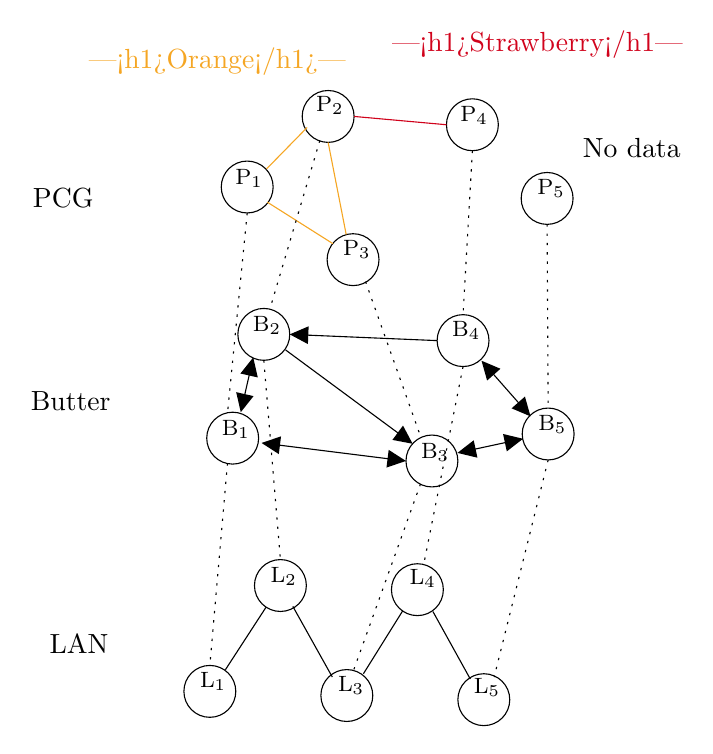
\begin{tikzpicture}[x=0.75pt,y=0.75pt,yscale=-1,xscale=1]
%uncomment if require: \path (0,451); %set diagram left start at 0, and has height of 451

%Shape: Circle [id:dp6061502443078786] 
\draw   (111,287.5) .. controls (111,280.6) and (116.6,275) .. (123.5,275) .. controls (130.4,275) and (136,280.6) .. (136,287.5) .. controls (136,294.4) and (130.4,300) .. (123.5,300) .. controls (116.6,300) and (111,294.4) .. (111,287.5) -- cycle ;
%Shape: Circle [id:dp36264343921365794] 
\draw   (126,237.5) .. controls (126,230.6) and (131.6,225) .. (138.5,225) .. controls (145.4,225) and (151,230.6) .. (151,237.5) .. controls (151,244.4) and (145.4,250) .. (138.5,250) .. controls (131.6,250) and (126,244.4) .. (126,237.5) -- cycle ;
%Shape: Circle [id:dp9971317502608965] 
\draw   (222,240.5) .. controls (222,233.6) and (227.6,228) .. (234.5,228) .. controls (241.4,228) and (247,233.6) .. (247,240.5) .. controls (247,247.4) and (241.4,253) .. (234.5,253) .. controls (227.6,253) and (222,247.4) .. (222,240.5) -- cycle ;
%Shape: Circle [id:dp9106166132377405] 
\draw   (263,285.5) .. controls (263,278.6) and (268.6,273) .. (275.5,273) .. controls (282.4,273) and (288,278.6) .. (288,285.5) .. controls (288,292.4) and (282.4,298) .. (275.5,298) .. controls (268.6,298) and (263,292.4) .. (263,285.5) -- cycle ;
%Shape: Circle [id:dp5541002056383258] 
\draw   (207,298.5) .. controls (207,291.6) and (212.6,286) .. (219.5,286) .. controls (226.4,286) and (232,291.6) .. (232,298.5) .. controls (232,305.4) and (226.4,311) .. (219.5,311) .. controls (212.6,311) and (207,305.4) .. (207,298.5) -- cycle ;
%Straight Lines [id:da3029168780037723] 
\draw    (154,237.63) -- (222,240.5) ;
\draw [shift={(151,237.5)}, rotate = 2.42] [fill={rgb, 255:red, 0; green, 0; blue, 0 }  ][line width=0.08]  [draw opacity=0] (8.93,-4.29) -- (0,0) -- (8.93,4.29) -- cycle    ;
%Straight Lines [id:da46957863774592223] 
\draw    (207.79,288.42) -- (149,245) ;
\draw [shift={(210.2,290.2)}, rotate = 216.45] [fill={rgb, 255:red, 0; green, 0; blue, 0 }  ][line width=0.08]  [draw opacity=0] (8.93,-4.29) -- (0,0) -- (8.93,4.29) -- cycle    ;
%Straight Lines [id:da9097415304582196] 
\draw    (245.38,252.45) -- (265.02,274.75) ;
\draw [shift={(267,277)}, rotate = 228.63] [fill={rgb, 255:red, 0; green, 0; blue, 0 }  ][line width=0.08]  [draw opacity=0] (8.93,-4.29) -- (0,0) -- (8.93,4.29) -- cycle    ;
\draw [shift={(243.4,250.2)}, rotate = 48.63] [fill={rgb, 255:red, 0; green, 0; blue, 0 }  ][line width=0.08]  [draw opacity=0] (8.93,-4.29) -- (0,0) -- (8.93,4.29) -- cycle    ;
%Straight Lines [id:da2061802483174313] 
\draw    (140.38,290.17) -- (204.02,298.13) ;
\draw [shift={(207,298.5)}, rotate = 187.13] [fill={rgb, 255:red, 0; green, 0; blue, 0 }  ][line width=0.08]  [draw opacity=0] (8.93,-4.29) -- (0,0) -- (8.93,4.29) -- cycle    ;
\draw [shift={(137.4,289.8)}, rotate = 7.13] [fill={rgb, 255:red, 0; green, 0; blue, 0 }  ][line width=0.08]  [draw opacity=0] (8.93,-4.29) -- (0,0) -- (8.93,4.29) -- cycle    ;
%Straight Lines [id:da9316247214989568] 
\draw    (234.73,293.97) -- (260.47,288.43) ;
\draw [shift={(263.4,287.8)}, rotate = 167.86] [fill={rgb, 255:red, 0; green, 0; blue, 0 }  ][line width=0.08]  [draw opacity=0] (8.93,-4.29) -- (0,0) -- (8.93,4.29) -- cycle    ;
\draw [shift={(231.8,294.6)}, rotate = 347.86] [fill={rgb, 255:red, 0; green, 0; blue, 0 }  ][line width=0.08]  [draw opacity=0] (8.93,-4.29) -- (0,0) -- (8.93,4.29) -- cycle    ;
%Straight Lines [id:da31757544534246873] 
\draw    (132.74,251.53) -- (128.06,272.07) ;
\draw [shift={(127.4,275)}, rotate = 282.8] [fill={rgb, 255:red, 0; green, 0; blue, 0 }  ][line width=0.08]  [draw opacity=0] (8.93,-4.29) -- (0,0) -- (8.93,4.29) -- cycle    ;
\draw [shift={(133.4,248.6)}, rotate = 102.8] [fill={rgb, 255:red, 0; green, 0; blue, 0 }  ][line width=0.08]  [draw opacity=0] (8.93,-4.29) -- (0,0) -- (8.93,4.29) -- cycle    ;
%Shape: Circle [id:dp39230600009532957] 
\draw   (100,409.5) .. controls (100,402.6) and (105.6,397) .. (112.5,397) .. controls (119.4,397) and (125,402.6) .. (125,409.5) .. controls (125,416.4) and (119.4,422) .. (112.5,422) .. controls (105.6,422) and (100,416.4) .. (100,409.5) -- cycle ;
%Shape: Circle [id:dp6725211407093591] 
\draw   (134,358.5) .. controls (134,351.6) and (139.6,346) .. (146.5,346) .. controls (153.4,346) and (159,351.6) .. (159,358.5) .. controls (159,365.4) and (153.4,371) .. (146.5,371) .. controls (139.6,371) and (134,365.4) .. (134,358.5) -- cycle ;
%Shape: Circle [id:dp534352110903068] 
\draw   (200,360.5) .. controls (200,353.6) and (205.6,348) .. (212.5,348) .. controls (219.4,348) and (225,353.6) .. (225,360.5) .. controls (225,367.4) and (219.4,373) .. (212.5,373) .. controls (205.6,373) and (200,367.4) .. (200,360.5) -- cycle ;
%Shape: Circle [id:dp5705459677432333] 
\draw   (232,413.5) .. controls (232,406.6) and (237.6,401) .. (244.5,401) .. controls (251.4,401) and (257,406.6) .. (257,413.5) .. controls (257,420.4) and (251.4,426) .. (244.5,426) .. controls (237.6,426) and (232,420.4) .. (232,413.5) -- cycle ;
%Shape: Circle [id:dp4884732451202879] 
\draw   (166,411.5) .. controls (166,404.6) and (171.6,399) .. (178.5,399) .. controls (185.4,399) and (191,404.6) .. (191,411.5) .. controls (191,418.4) and (185.4,424) .. (178.5,424) .. controls (171.6,424) and (166,418.4) .. (166,411.5) -- cycle ;
%Straight Lines [id:da5435068621925384] 
\draw    (139.5,369.07) -- (120,399.07) ;
%Straight Lines [id:da40058310101255523] 
\draw    (152.5,368.57) -- (171.5,402.57) ;
%Straight Lines [id:da745960373491508] 
\draw    (205.5,370.57) -- (186.5,401) ;
%Straight Lines [id:da9636103089067328] 
\draw    (220,371.07) -- (238,403.57) ;
%Straight Lines [id:da026025176740933853] 
\draw  [dash pattern={on 0.84pt off 2.51pt}]  (121,299.57) -- (112.5,397) ;
%Straight Lines [id:da8574677477453254] 
\draw  [dash pattern={on 0.84pt off 2.51pt}]  (138.5,250) -- (146.5,346) ;
%Straight Lines [id:da45830762125909896] 
\draw  [dash pattern={on 0.84pt off 2.51pt}]  (234.5,253) -- (215.5,348.57) ;
%Straight Lines [id:da692101028265002] 
\draw  [dash pattern={on 0.84pt off 2.51pt}]  (214,309.57) -- (181.5,400.07) ;
%Straight Lines [id:da20439957038676881] 
\draw  [dash pattern={on 0.84pt off 2.51pt}]  (275.5,298) -- (249.5,402.57) ;
%Shape: Circle [id:dp24822651082567027] 
\draw  [color={rgb, 255:red, 0; green, 0; blue, 0 }  ,draw opacity=1 ] (118,166.5) .. controls (118,159.6) and (123.6,154) .. (130.5,154) .. controls (137.4,154) and (143,159.6) .. (143,166.5) .. controls (143,173.4) and (137.4,179) .. (130.5,179) .. controls (123.6,179) and (118,173.4) .. (118,166.5) -- cycle ;
%Shape: Circle [id:dp425639162940066] 
\draw  [color={rgb, 255:red, 0; green, 0; blue, 0 }  ,draw opacity=1 ] (157,132.5) .. controls (157,125.6) and (162.6,120) .. (169.5,120) .. controls (176.4,120) and (182,125.6) .. (182,132.5) .. controls (182,139.4) and (176.4,145) .. (169.5,145) .. controls (162.6,145) and (157,139.4) .. (157,132.5) -- cycle ;
%Shape: Circle [id:dp15558332675817688] 
\draw  [color={rgb, 255:red, 0; green, 0; blue, 0 }  ,draw opacity=1 ] (169,201.5) .. controls (169,194.6) and (174.6,189) .. (181.5,189) .. controls (188.4,189) and (194,194.6) .. (194,201.5) .. controls (194,208.4) and (188.4,214) .. (181.5,214) .. controls (174.6,214) and (169,208.4) .. (169,201.5) -- cycle ;
%Shape: Circle [id:dp30081719961232734] 
\draw   (226.5,136.5) .. controls (226.5,129.6) and (232.1,124) .. (239,124) .. controls (245.9,124) and (251.5,129.6) .. (251.5,136.5) .. controls (251.5,143.4) and (245.9,149) .. (239,149) .. controls (232.1,149) and (226.5,143.4) .. (226.5,136.5) -- cycle ;
%Straight Lines [id:da8972847915279969] 
\draw [color={rgb, 255:red, 245; green, 166; blue, 35 }  ,draw opacity=1 ]   (139.8,157.8) -- (159.4,137.8) ;
%Straight Lines [id:da4060630063522047] 
\draw [color={rgb, 255:red, 245; green, 166; blue, 35 }  ,draw opacity=1 ]   (178.2,189.4) -- (169.5,145) ;
%Straight Lines [id:da6848460896070612] 
\draw [color={rgb, 255:red, 245; green, 166; blue, 35 }  ,draw opacity=1 ]   (140.2,173.8) -- (171.8,193.8) ;
%Straight Lines [id:da5819580495505107] 
\draw [color={rgb, 255:red, 208; green, 2; blue, 27 }  ,draw opacity=1 ]   (182,132.5) -- (226.5,136.5) ;
%Straight Lines [id:da49699117013802474] 
\draw  [dash pattern={on 0.84pt off 2.51pt}]  (130.5,179) -- (121,275.57) ;
%Straight Lines [id:da5794423519351266] 
\draw  [dash pattern={on 0.84pt off 2.51pt}]  (165.5,144.07) -- (141.5,225.07) ;
%Straight Lines [id:da9796158041739726] 
\draw  [dash pattern={on 0.84pt off 2.51pt}]  (187.5,212.07) -- (214,286.57) ;
%Straight Lines [id:da23772443967474888] 
\draw  [dash pattern={on 0.84pt off 2.51pt}]  (239,149) -- (234.5,228) ;
%Shape: Circle [id:dp47924057339080184] 
\draw   (262.5,172) .. controls (262.5,165.1) and (268.1,159.5) .. (275,159.5) .. controls (281.9,159.5) and (287.5,165.1) .. (287.5,172) .. controls (287.5,178.9) and (281.9,184.5) .. (275,184.5) .. controls (268.1,184.5) and (262.5,178.9) .. (262.5,172) -- cycle ;
%Straight Lines [id:da813689736444334] 
\draw  [dash pattern={on 0.84pt off 2.51pt}]  (275,184.5) -- (275.5,273) ;

% Text Node
\draw (26,166) node [anchor=north west][inner sep=0.75pt]   [align=left] {PCG};
% Text Node
\draw (34,381) node [anchor=north west][inner sep=0.75pt]   [align=left] {LAN};
% Text Node
\draw (25,264) node [anchor=north west][inner sep=0.75pt]   [align=left] {Butter};
% Text Node
\draw (53,98) node [anchor=north west][inner sep=0.75pt]   [align=left] {\textcolor[rgb]{0.96,0.65,0.14}{\lstinline|<h1>Orange</h1>|}};
% Text Node
\draw (199,90) node [anchor=north west][inner sep=0.75pt]   [align=left] {\textcolor[rgb]{0.82,0.01,0.11}{\lstinline|<h1>Strawberry</h1|}};
% Text Node
\draw (123.5,156.57) node [anchor=north west][inner sep=0.75pt]   [align=left] {{\footnotesize P\textsubscript{1}}};
% Text Node
\draw (162.5,121.57) node [anchor=north west][inner sep=0.75pt]   [align=left] {{\footnotesize P\textsubscript{2}}};
% Text Node
\draw (232,126.57) node [anchor=north west][inner sep=0.75pt]   [align=left] {{\footnotesize P\textsubscript{4}}};
% Text Node
\draw (269,161.57) node [anchor=north west][inner sep=0.75pt]   [align=left] {{\footnotesize P\textsubscript{5}}};
% Text Node
\draw (175.5,191.07) node [anchor=north west][inner sep=0.75pt]   [align=left] {{\footnotesize P\textsubscript{3}}};
% Text Node
\draw (117,277.57) node [anchor=north west][inner sep=0.75pt]   [align=left] {{\footnotesize B\textsubscript{1}}};
% Text Node
\draw (132,227.57) node [anchor=north west][inner sep=0.75pt]   [align=left] {{\footnotesize B\textsubscript{2}}};
% Text Node
\draw (213,288.57) node [anchor=north west][inner sep=0.75pt]   [align=left] {{\footnotesize B\textsubscript{3}}};
% Text Node
\draw (228,230.07) node [anchor=north west][inner sep=0.75pt]   [align=left] {{\footnotesize B\textsubscript{4}}};
% Text Node
\draw (269.5,275.07) node [anchor=north west][inner sep=0.75pt]   [align=left] {{\footnotesize B\textsubscript{5}}};
% Text Node
\draw (291,141.57) node [anchor=north west][inner sep=0.75pt]   [align=left] {No data};
% Text Node
\draw (106.5,399.07) node [anchor=north west][inner sep=0.75pt]   [align=left] {{\footnotesize L\textsubscript{1}}};
% Text Node
\draw (140.5,348.57) node [anchor=north west][inner sep=0.75pt]   [align=left] {{\footnotesize L\textsubscript{2}}};
% Text Node
\draw (173,401.07) node [anchor=north west][inner sep=0.75pt]   [align=left] {{\footnotesize L\textsubscript{3}}};
% Text Node
\draw (207.5,349.5) node [anchor=north west][inner sep=0.75pt]   [align=left] {{\footnotesize L\textsubscript{4}}};
% Text Node
\draw (238.5,402.07) node [anchor=north west][inner sep=0.75pt]   [align=left] {{\footnotesize L\textsubscript{5}}};


\end{tikzpicture}

    \caption{Example overlay structure with PCG}
    \label{fig:overlayPCG}
\end{figure}

% This is a illustrated example
Figure~\ref{fig:overlayPCG} illustrates an instance of a Butter network with a PCG overlay. In this example we see an underlying LAN network where the edges represent physical or local WIFI connections. The directed edges at the Butter level represent a node's known hosts and the edges in PCG layer represent group members.

The group of $P_1$, $P_2$ and $P_3$ are responsible for maintaining the information for the ``Orange" webpage. In the case that $r=3$ they are a complete group. The group $P_2$ and $P_4$ is responsible for ``Strawberry" but is in a cold state. In a cold state, a leader is elected amongst the two nodes and his responsibility is to find a node in his known hosts that is able to participate in the group. In this case, say that $P_4$ is elected leader, he interacts with the underlying butter node $B_4$ and sees that he has available known hosts $B_2$ and $B_5$. Say $B_5$ is asked to join the group, if it has the available storage, it will join and complete the group.

%\subsubsection{Request handler}
%
%A key feature of the original PCG implementation is that it allows for transparent content delivery despite high churn\cite{shinebourne2022availability}. All group members are responsible for responding to a request for information, and hence the burden does not fall on a specific node. This allows a request to be fulfilled despite the failure of the initial node responding to the request as if the initial peer fails, another peer will fulfil it. This has benefits for ease of implementation on the client side as there is no need to handle re-attempting to query the network for information if a request is unfinished, but has major drawbacks with network utilisation and implementation complexity. Therefore, Butter does not include this transparent interface and puts the responsibility of fulfilling a request on the client asking for the information. In other words, it is the client's responsibility to work to retrieve data, not that of the network.

\subsubsection{Extra optimisation}

% Geographic distribution
A $geo$ tag can be appended to each node's known host quality metric so when a leader is elected to find a new peer to join the group (if the group is deemed to be in an unsafe state) it will favour picking nodes with different $geo$ tags. This attempts to maximise the probability of redundant copies of information being distributed geographically, resulting in less shared infrastructure and improved information retrieval by reducing the average latency and steps taken to discover data.

\subsection{Testing \& evaluation}

In this section we will discuss how the design was tested as well as the different relationships between parameters such as heartbeat intervals and replication count. Based on the tests we evaluate the design and discuss some of the benefits and shortfalls of the implementation as well as what could be improved in future iterations.

\subsubsection{Methodology}
\label{sec:churnTesting}

The testing process is carries out as follows:

\begin{enumerate}
    \item The testbed generates $n$ nodes on different ports, each tasked with storing a random string of data.
    \item Test waits for nodes to spawn and form a network
    \item $chanceToDie$ and $churnTime$ parameters are specified. The $chanceToDie$ determines the probability that a node is terminated during the $churnTime$.
    \item Testbed churns the network and so simulates nodes failing over time. During churn new nodes are created to maintain the network node count at $n$.
    \item The network is left a moment to recover, allowing the remaining nodes to re-create and update their list of known hosts. New nodes are created to replace failed nodes, in order to maintain the number of nodes on the network.
    \item After a given period of time has passed, a new querying node is created with a list of all of the identifiers for information initially added to the network. The querying node attempts to retrieve all of the data that was initially stored in the network during initialisation. This node takes count of the number of successful and failed information queries, and so can provide a metric of the proportion of data that persisted on the network `post-churn'. The information retrieval algorithm used by the querying node is BFS (more on this in Section~\ref{sec:ir}). BFS allows for thorough exploration of the network so that we can be certain that the information is no present.
\end{enumerate}

% In addition, there is a centralised logging node used in development logging mode where peers frequently publish their stats to a centralised server which updates a database of nodes, their edges, properties and information they contaain - this allows for a visualisation of the current state of the network. It is important to note that this centralised server does not carry out any functionality and is simply used for logging the network. If nodes are unable to publish to the server they simply try again - publishing to the server cannot cause failure meaning that sometimes the loging can be incorrect.

\subsubsection{Results \& evaluation}

\begin{table}[ht]
    \centering
    \begin{tabular}{|l|l|l|}
        \hline
        Heartbeat interval (s) & Nb. messages sent & (\%) Success rate \\
        \hline
        10                     & 600               & 58.00             \\
        5                      & 1200              & 60.00             \\
        2                      & 3000              & 72.00             \\
        1                      & 6000              & 74.00             \\
        \hline
    \end{tabular}
    \caption{Experimental data from test rig. Tested on 100 simulated nodes, repeated 5 times at each heartbeat interval setting. \textbf{Note}: Messages sent is the cumulative amount of heartbeat messages sent between group participants over a 60s churn time, $chanceToDie$ was set to 1 in 50 across all heartbeat intervals.}
    \label{tab:heartbeatSuccess}
\end{table}

There were some initial issues with testing due to the speed of churn in simulation relative to the speed at which the nodes were carrying out heartbeats, i.e.\ the simulated churn rate was extremely high and heartbeat intervals too far apart. This was resolved by changing the heartbeat interval from 10s to 2s. This does increase the message complexity of the network greatly and so in practice the parameter should be considered carefully, based on the specifics of the network.

To demonstrate how message complexity scales with different heartbeat intervals and how heartbeat intervals influence information retention we can observe the data in Table~\ref{tab:heartbeatSuccess}. For a short interval $t_h$ (e.g.\ 1 or 2 seconds), the probability of all peers maintaining some data $X$ failing in between $t_h+t_r$ where $t_r$ is the time to recover to $n=r$, is very low. However, this requires the node to constantly flood the group with heartbeat queries and hence scales poorly.

%In the testing environment, we found 2 second heartbeat intervals to be a good compromise between maintaining groups effectively while reducing the heartbeat messages sent by a factor of 2 from a 1s heartbeat interval. This is an appropriate setting in the testing environment, however, in reality a greater heartbeat interval may be preferred as the churn rate may be less high in other practical instances of Butter networks.

When the initial tests were carried out\cite{shinebourne2022availability}, success rate was lower than expected. This turned out to be because heartbeat intervals were all in sync and hence inspired the design for heartbeat palpitations. Once palpitations were introduced and hence the intervals offset, success rate improved greatly.

\begin{table}[ht]
    \centering
    \begin{tabular}{|l|l|l|}
        \hline
        $chanceToDie$ & Nb. failed to retrieve & (\%) Success rate \\
        \hline
        1 in 50       & 63                     & 74.80             \\
        1 in 100      & 29                     & 88.40             \\
        1 in 1000     & 4                      & 98.40             \\
        1 in 10,000   & 0                      & 100.00            \\
        \hline
    \end{tabular}
    \caption{Experimental data collected from testbed. Tested on 250 simulated nodes, repeated 5 times at each $chanceToDie$; average is rounded to the closest node. \textbf{Note}: the $chanceToDie$ is per second, the network churn time was 30s and the heartbeats were set to every 2s.}
    \label{tab:chanceToDieResults}
\end{table}

In an effort to help interpret the data in Table~\ref{tab:chanceToDieResults}, think about the probability of an initially spawned node surviving churn when the $chanceToDie$ is 1 in 50. In that case, every second, for 30 seconds, each of the 250 nodes has a 1 in 50 chance of dying. In other words, for every second there is a $49/50$ chance of survival to the next second. The probability, therefore, of an initially spawned node surviving the churn stage of the testing process is $(\frac{49}{50})^{30}=0.545$. So, with a 1 in 50 $chanceToDie$, we can expect just above half the network to have failed over the course of the churn. With the persistent storage mechanism we have managed to retain on average 74.80\% of the original information. While this is not a perfect solution, it shows a significant improvement in terms of availability. The tests stressed the importance of choosing an appropriate heartbeat interval.

%\begin{table}[ht]
%    \centering
%    \begin{tabular}{|l|l|l|}
%        \hline
%        Group size & Nb. messages sent & (\%) Success rate \\
%        \hline
%        3          & 3000                & 74.80             \\
%        5          & 29                & 88.40             \\
%        10         & 4                 & 98.40             \\
%        \hline
%    \end{tabular}
%    \caption{Experimental data collected from test rig. Tested on 100 simulated nodes. \textbf{Note}: Chance to die was set to 1 in 100 and the heartbeat interval was set to 2s.}
%    \label{tab:group_size_results}
%\end{table}
%
%
%Finally, a last set of tests were carried out to provide insights into optimal group size. The group size can be user specified, and should be set cautiously, much like the heartbeat interval. Groups need to be sufficiently large so as to increase the probability of data retention but also small enough to make group maintenance efficient. As Table~\ref{tab:group_size_results} shows, group size will has a substantial effect on the amount of messages sent. Heartbeat may work for small group sizes but will not be suitable for larger groups.

Having carried out testing we can consider that the implemented solution has succeeded in providing a certain level of data persistence across a decentralised peer-to-peer network. Despite the limitations of the testbed, Table~\ref{tab:chanceToDieResults} shows that a significant amount of information that would otherwise have been lost, if no mechanisms for data persistence existed, was still present in the network after a period of relatively high simulated network churn.

An interesting future development might be to introduce dynamic group sizes\cite{ramaswamy2005clustering}. The groups and hence redundant copies of the data could dynamically grow with the popularity, i.e.\ frequency of access of a piece of information. This may improve availability for popular information, but more importantly, it would spread the load of information requests ensuring that average file download latency does not increase significantly for highly desired information. In addition it could increase the probability of $QUERYHIT$s in information retrieval. This will be further discussed in Section~\ref{sec:ir}.

Finally, PCG provides an elegant way of reasoning about persistent information on the network. The extension of PCG developed here improves the fault-tolerance and scalability of the original design by taking away some of the aspects that introduce centralisation, i.e.\ the publishing rendezvous super-peers. However, there is still a significant drawback in message complexity that will need to be addressed for networks at scale. A better future implementation may involve implementing randomised gossiping to solve the GMP, however, more testing will be needed.



